\documentclass{beamer}
%Imports and customization
\usepackage{tikz}
\usepackage{graphicx}
\usepackage{tikz-feynman}
\graphicspath{ 
    {./images/}
}

\beamertemplatenavigationsymbolsempty
\setbeamertemplate{sidebar right}{}
\setbeamertemplate{footline}{
    \hfill\usebeamertemplate***{navigation symbols}
    \hspace{1cm}\insertframenumber{}/\inserttotalframenumber
}
\setbeamertemplate{caption}{\raggedright\insertcaption\par}
\setbeamersize{text margin left=5mm,text margin right=5mm} 

\setbeamerfont{itemize/enumerate body}{size=\scriptsize}
\setbeamerfont{itemize/enumerate subbody}{size=\scriptsize}
\setbeamerfont{itemize/enumerate subsubbody}{size=\scriptsize}


%Custom Macros
\newcommand{\statwarn}{
    \tiny \color{red} Absolute numbers here mean NOTHING. Plots are based on small (100k events) samples, and are highly biased. All that matters is relative position!
}


\newcommand{\fullscreenimage}[2]{
    \frame{
        \frametitle{#1} 
        \begin{figure}
        \includegraphics[height=0.9\textheight,keepaspectratio]{#2}
        \end{figure}
    }
}


\newcommand{\displayone}[3]{
    \frame{
        \frametitle{#1} 
        \begin{columns}
            \begin{column}{0.5\textwidth}
                #2
            \end{column}
            \begin{column}{0.5\textwidth}
                \begin{figure}
                    \includegraphics[width=\linewidth,height=\textheight,keepaspectratio]{#3}
                \end{figure}
            \end{column}
        \end{columns}
    }
}

\newcommand{\displayonelarge}[3]{
    \frame{
        \frametitle{#1} 
        \begin{columns}
            \begin{column}{0.3\textwidth}
                #2
            \end{column}
            \begin{column}{0.7\textwidth}
                \begin{figure}
                    \includegraphics[width=\linewidth,height=\textheight,keepaspectratio]{#3}
                \end{figure}
            \end{column}
        \end{columns}
    }
}


\newcommand{\displaytwo}[4]{
    \frame{
        \frametitle{#1} 
        #2
        \begin{columns}
            \begin{column}{0.5\textwidth}
                \begin{figure}
                    \includegraphics[width=\linewidth,height=\textheight,keepaspectratio]{#3}
                \end{figure}
            \end{column}
            \begin{column}{0.5\textwidth}
                \begin{figure}
                    \includegraphics[width=\linewidth,height=\textheight,keepaspectratio]{#4}
                \end{figure}
            \end{column}
        \end{columns}
    }
}


\newcommand{\displaythree}[5]{
    \frame{
        \begin{columns}[T]
            \begin{column}{0.5\textwidth}
                \insertframetitle{#1}\\
                #2
            \end{column}
            \begin{column}{0.5\textwidth}
                \begin{figure}
                    \includegraphics[width=\linewidth,height=\textheight,keepaspectratio]{#3}
                \end{figure}
            \end{column}
        \end{columns}
        \begin{columns}[T]
            \begin{column}{0.5\textwidth}
                \begin{figure}
                    \includegraphics[width=\linewidth,height=\textheight,keepaspectratio]{#4}
                \end{figure}
            \end{column}
            \begin{column}{0.5\textwidth}
                \begin{figure}
                    \includegraphics[width=\linewidth,height=\textheight,keepaspectratio]{#5}
                \end{figure}
            \end{column}
        \end{columns}
    }
}


\newcommand{\announcesection}[1]{
    \section{#1}
    \frame{
        \begin{center}
            {\huge #1} 
        \end{center}
    }
}


%Begin Presentation
\begin{document}
    \title{ Status Report: VBF/ggF Separation in Di-Higgs }
    \author{Chris Milke}
    \date{13 July, 2020}

    \frame{\titlepage}
    \frame{\frametitle{Overview} \tableofcontents}

    \fullscreenimage{VBF Di-Higgs Analysis}{vbf-hh_diagrams}
\frame{
    \frametitle{ VBF $\rightarrow$ HH $\rightarrow$ \fourB }

    \begin{columns}
        \begin{column}{0.5\textwidth}
            { \small
                Goal is to put a better limit on the $C_{2V}$ coupling constant.
            }

            \begin{figure}
                \includegraphics[width=\linewidth,height=\textheight,keepaspectratio]
                {dihiggs_task_list}
            \end{figure}
        \end{column}
        \begin{column}{0.5\textwidth}
            \resizebox{0.50\textheight}{!}{
                \begin{tikzpicture} \begin{feynman}
    \vertex (c2v) {\tiny $C_{2V}$};
    \vertex [above right=of c2v] (h1) {H};
    \vertex [below right=of c2v] (h2) {H};
    \vertex [above left=of c2v] (vb1);
    \vertex [below left=of c2v] (vb2);
    \vertex [left=of vb1] (q1i) {q};
    \vertex [left=of vb2] (q2i) {q};
    \vertex [above right=of h1] (b1) {$b$};
    \vertex [below right=of h2] (bbar2) {$\bar b$};
    \vertex [below=of b1] (bbar1) {$\bar b$};
    \vertex [above=of bbar2] (b2) {$b$};

    \vertex [above=of b1] (q1f) {q};
    \vertex [below=of bbar2] (q2f) {q};

    \diagram* {
        (q1i) -- (vb1) -- (q1f),
        (q2i) -- (vb2) -- (q2f), 
        (vb1) -- [boson] (c2v) -- [boson] (vb2),
        (h1) -- [scalar] (c2v) -- [scalar] (h2),
        (b1) -- (h1) -- (bbar1),
        (b2) -- (h2) -- (bbar2),
    };
\end{feynman} \end{tikzpicture}

            }
        \end{column}
    \end{columns}
}

    \section{Analysis Baseline Status}

\displayonelarge{VBF Selection Process Overview}{
    Selection of VBF events from data is done through a series of selection "filters"
}{cutflows/general}

\displayonelarge{VBF-Specific Selections}{
    {\tiny \begin{itemize}
        \item VBF Pair: Remove events in which there are fewer than two jets that are {\bf not} btagged
        \item VBF dEta: Select the jet pair with the highest invariant mass as the  "VBF Pair".\\Remove events where the $\Delta \eta$ of this pair is less than 3
        \item VBF mjj: Remove events where the "VBF Pair's" invariant mass is less than 1000 GeV
    \end{itemize} }
}{cutflows/vbf_only}

\displaytwo{ggF vs VBF for Various \cvv Values}{
    Current selection process across ggF and varying values of \cvv
}{cutflows/c2v_compare}{cutflows/c2v_compare_log}

    \fullscreenimage{ROC Curves! (They're Not Going Away!)}{rocs/roc_explanation}
    \section{BDT Improvements}

\displayonelarge{From Last Time: My Initial Attempt at BDTs}{
    {\small My first attempts at a BDT were very rudimentary, using improper weighting, basic kinematic variables as inputs and poor statistics.}

    \vspace{10mm}

    {\tiny *BDT is trained using SKLearn, with inputs:}
    \begin{itemize}
        {\tiny \item $p_T$ of 2 leading-$p_T$ jets }
        {\tiny \item $\eta$ of 2 leading-$p_T$ jets }
        {\tiny \item $\phi$ of 2 leading-$p_T$ jets }
        {\tiny \item $Energy$ of 2 leading-$p_T$ jets }
        {\tiny \item $M_{jj}$ of leading $M_{jj}$ pair }
    \end{itemize}
}{rocs/first_roc}

\displayonelarge{Step 1: Actually Tell SK-Learn that Samples are Weighted}{
    As a baseline, train BDT with same inputs as current algorithm. It should perform at least as well.
}{rocs/baseline_roc}

\displayfour{Step 2: Improve Inputs - Fox Wolfram Moments}
{fw_moments/fox-wolfram_1}
{fw_moments/fox-wolfram_2}
{fw_moments/fox-wolfram_3}
{fw_moments/fox-wolfram_4}

\displaytwo{BDT with Fox-Wolfram Moments}{
    Improvent from first seven FW Moments is minor, but noticeable.
}{rocs/rocs_bdt2}{rocs/rocs_bdt2_zoom}


\displayonelarge{Step 3: Increase Statistics Using Cross Validation}{
    {\small Switching to TMVA and utilizing cross validation training improves performance with the same BDT inputs and architecture.
    Opens the door for more complex BDT architectures.}
}{rocs/rocs_cross_validation}



    \fullscreenimage{Comparing Selection Performance}{roc_explanation}
\fullscreenimage{Current Selection Method Performance}{rocs/rocs_initial}

\displayonelarge{Baseline BDT}{
    As a baseline, train BDT with same inputs as current algorithm. It should perform at least as well.
}{rocs/rocs_bdt1}

\fullscreenimage{Adding Fox-Wolfram Moments to BDT}{fwMoment_ordering}
\displayfour{Fox-Wolfram Distributions}
{fw_moments/fox-wolfram_1}
{fw_moments/fox-wolfram_2}
{fw_moments/fox-wolfram_3}
{fw_moments/fox-wolfram_4}


\displaytwo{BDT with Fox-Wolfram Moments}{
    Improvent from first seven FW Moments is minor, but noticeable.
}{rocs/rocs_bdt2}{rocs/rocs_bdt2_zoom}


\frame{
    \frametitle{Exploring Multi-Jet Discriminants: Centrality}
    \begin{columns}
        \begin{column}{0.5\textwidth}
            {\small The VBF initial scatter quark jets are not always the only thing present in VBF events.
            Radiated Jets (ISR \& FSR) are not uncommon, and provide additional handles for analysis.}
            \begin{figure}
                \includegraphics[width=\linewidth,height=\textheight,keepaspectratio]{ event_display}
            \end{figure}
        \end{column}
        \begin{column}{0.5\textwidth}
            \begin{center}\resizebox{0.40\textheight}{!}{ 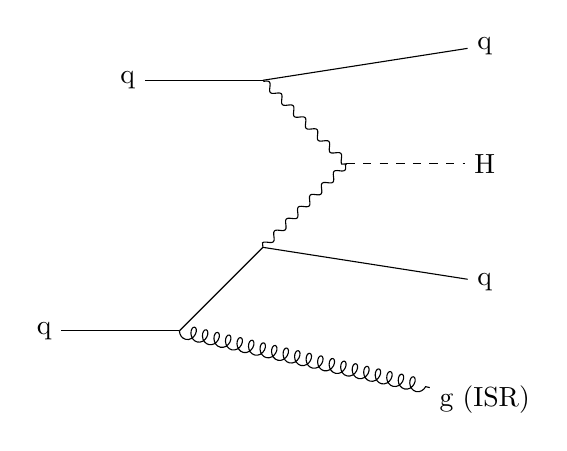
\begin{tikzpicture} \begin{feynman}
    \vertex (a);
    \vertex [right=of a] (b) {H};
    \vertex [above left=of a] (vb1);
    \vertex [below left=of a] (vb2);
    \vertex [left=of vb1] (q1i) {q};
    \vertex [below left=of vb2] (q2k);
    \vertex [left=of q2k] (q2i) {q};
    \vertex [above =of b] (q1f) {q};
    \vertex [below =of b] (q2f) {q};
    \vertex [below =of q2f] (g) {g (ISR)};

    \diagram* {
        (q1i) -- (vb1) -- (q1f),
        (q2i) -- (q2k) -- (vb2) -- (q2f),
        (q2k) --[gluon] (g),
        (vb1) -- [boson] (a) -- [boson] (vb2),
        (a) -- [scalar] (b),
    };
\end{feynman} \end{tikzpicture}
 }\end{center}
            \begin{center}\resizebox{0.40\textheight}{!}{ \begin{tikzpicture} \begin{feynman}
    \vertex (a);
    \vertex [right=of a] (b) {H};
    \vertex [above left=of a] (vb1);
    \vertex [below left=of a] (vb2);
    \vertex [left=of vb1] (q1i) {q};
    \vertex [left=of vb2] (q2i) {q};
    \vertex [below right=of vb2] (q2k);
    \vertex [above =of b] (q1f) {q};
    \vertex [below =of b] (q2f) {q};
    \vertex [below =of q2f] (g) {g (FSR)};

    \diagram* {
        (q1i) -- (vb1) -- (q1f),
        (q2i) -- (vb2) -- (q2k) -- (q2f), 
        (q2k) --[gluon] (g),
        (vb1) -- [boson] (a) -- [boson] (vb2),
        (a) -- [scalar] (b),
    };
\end{feynman} \end{tikzpicture}
 }\end{center}
        \end{column}
    \end{columns}
}


\fullscreenimage{Centrality Distribution}{centrality}
\displaytwo{Centrality as a BDT Input}{
    Improvement from Centrality is very small,
    but there may be more to be gained with further study.
}{rocs/rocs_centrality}{rocs/rocs_centrality_zoom0}



    \section{Conclusion}
    \frame{
        \frametitle{Conclusions}
        \begin{itemize} {
            \item Significant progress has been made in improving my VBF/ggF separation BDT
            \item Large scale view of the selection process is encouraging, with BDT showing promise of noticeably reducing ggF contamination
            \item Investigation into more complex inputs is ongoing, but will require involved technical work with underlying code-base
        } \end{itemize}
    }

    \announcesection{Backup}
    \fullscreenimage{}{Xwt_plots/final_weight_comparison_FourTagCutflow_with_cvv4}
    \fullscreenimage{}{Xwt_plots/final_weight_comparison_TwoTagCutflow}
    \fullscreenimage{}{Xwt_plots/final_roc_TwoTagCutflow}
    \input{fox_wolfram_dump.tex}
\end{document}
